
\chapter{Additional Deep-Dive Analysis of Experiment Runs}
\label{app:deep-dive-experiments}

This appendix intentionally collects more detail than the main thesis needs. It
is a staging area for exploratory analysis of the Runpod/W\&B vision runs and
the MLflow regression runs. The purpose is to expose patterns that may later be
pruned into the main text or converted into a smaller set of final figures.

\section{Regression continuation: quality--runtime trade-off}

Figure~\ref{fig:deep-regression-tradeoff} compares the median quality gain of
curriculum training against its runtime cost for the controlled
\texttt{curr\_vs\_single\_20260315\_175826} benchmark. The horizontal axis is
larger than one for every function and budget regime, which means that the
curriculum was always slower. The vertical axis is positive only when curriculum
reduced hard-validation loss.

\begin{figure}[h]
    \centering
    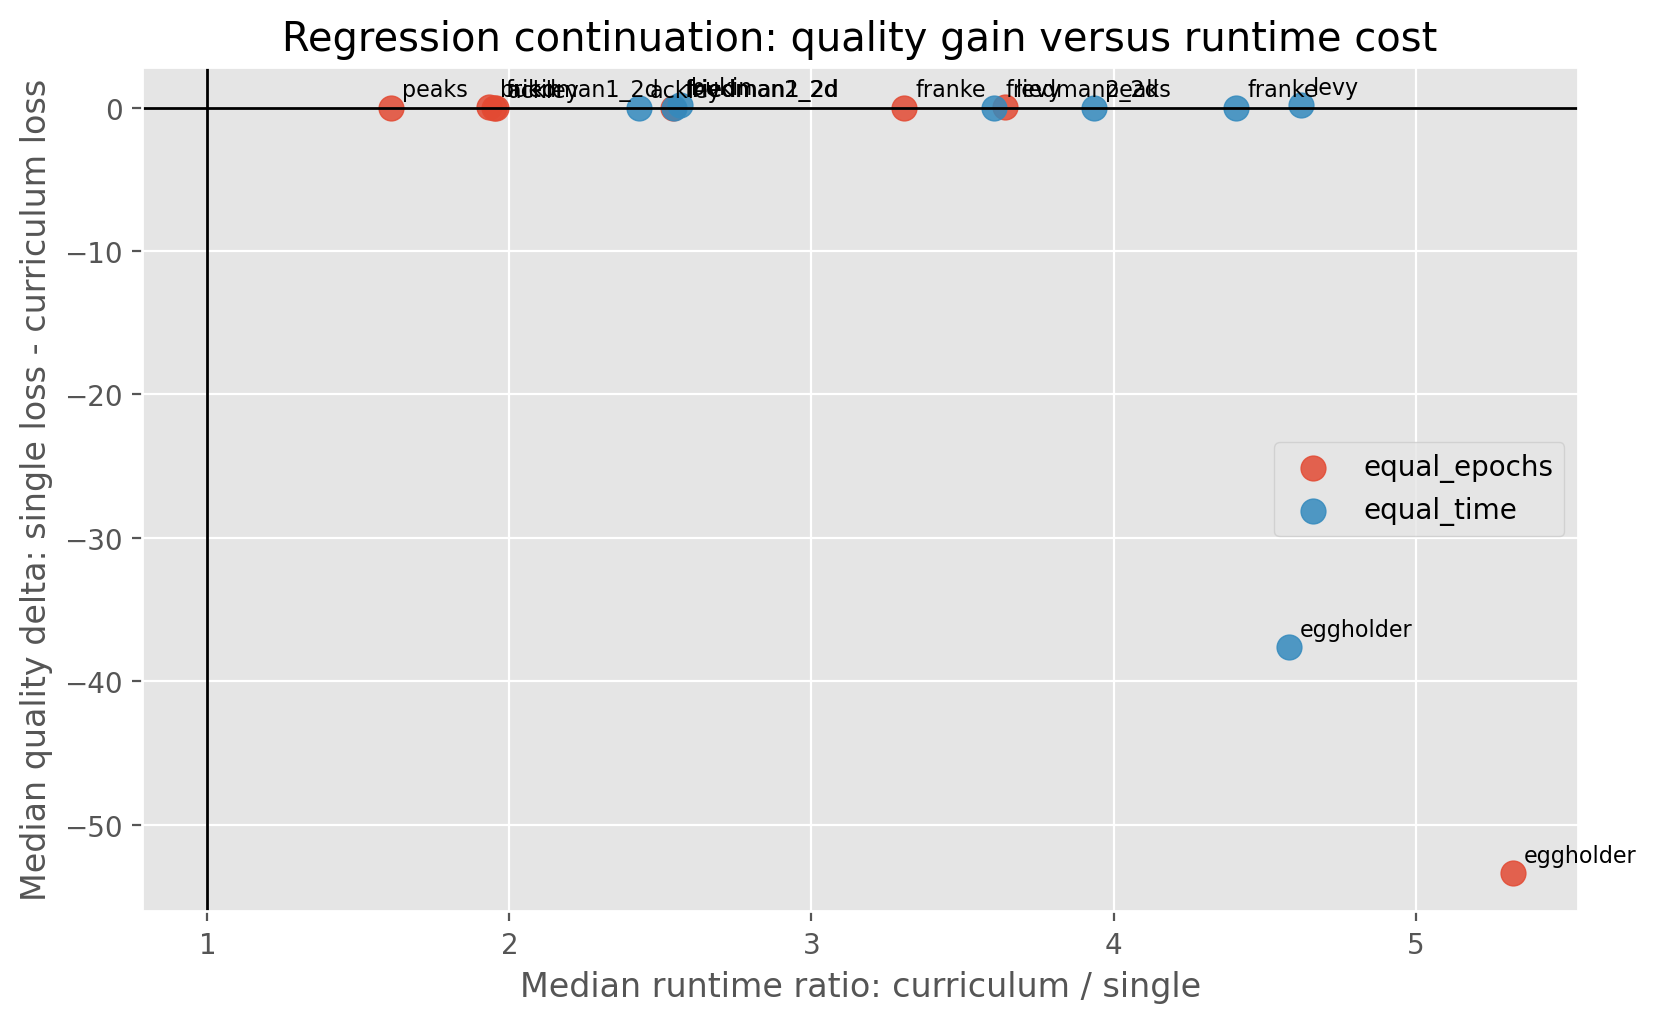
\includegraphics[width=0.86\textwidth]{figures/deep_regression_quality_runtime_tradeoff.png}
    \caption{Quality gain versus runtime cost for Gaussian-continuation
    regression. Positive y-values favor curriculum; x-values above one mean the
    curriculum run was slower than direct single-target training.}
    \label{fig:deep-regression-tradeoff}
\end{figure}

\begin{table}[h]
\centering
\small
\begin{tabular}{llrrl}
\toprule
Function & Regime & Quality delta & Runtime ratio & Winner \\
\midrule
ackley & equal\_epochs & -0.00762 & 1.96 & single \\
bukin & equal\_epochs & 0.032 & 1.93 & curriculum \\
eggholder & equal\_epochs & -53.4 & 5.32 & single \\
franke & equal\_epochs & 4.23e-06 & 3.31 & curriculum \\
friedman1\_2d & equal\_epochs & 0.000129 & 1.95 & curriculum \\
friedman2\_2d & equal\_epochs & 0.000462 & 2.54 & curriculum \\
levy & equal\_epochs & 0.0104 & 3.64 & curriculum \\
peaks & equal\_epochs & -0.00015 & 1.61 & single \\
ackley & equal\_time & -0.00286 & 2.43 & single \\
bukin & equal\_time & 0.176 & 2.57 & curriculum \\
eggholder & equal\_time & -37.6 & 4.58 & single \\
franke & equal\_time & 1.17e-05 & 4.41 & curriculum \\
friedman1\_2d & equal\_time & -4.78e-05 & 2.55 & single \\
friedman2\_2d & equal\_time & -7.34e-05 & 3.61 & single \\
levy & equal\_time & 0.169 & 4.62 & curriculum \\
peaks & equal\_time & -0.000236 & 3.94 & single \\
\bottomrule
\end{tabular}
\caption{Function-level regression deltas. Quality delta is median
single-target hard-validation loss minus median curriculum hard-validation loss,
so positive values favor curriculum. Runtime ratio is curriculum runtime divided
by single-target runtime.}
\label{tab:deep-regression-deltas}
\end{table}

Figure~\ref{fig:deep-regression-seed-heatmap} shows the same comparison after
pairing runs by seed. The sign pattern is not random: \texttt{bukin},
\texttt{franke}, and \texttt{levy} are the clearest positive cases, while
\texttt{ackley}, \texttt{eggholder}, and \texttt{peaks} are negative in
both budget regimes.

\begin{figure}[h]
    \centering
    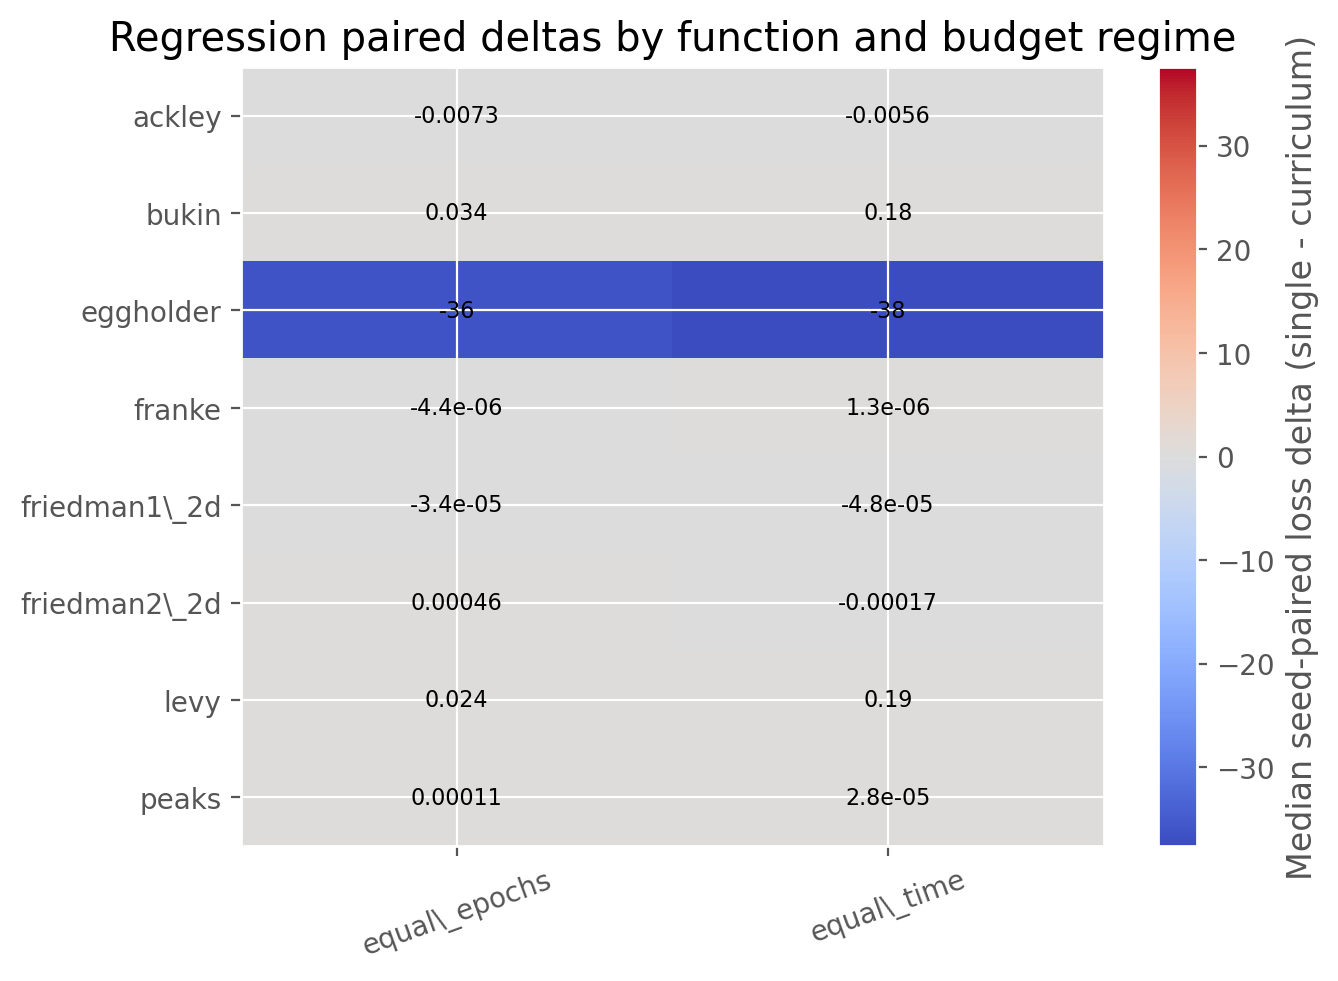
\includegraphics[width=0.72\textwidth]{figures/deep_regression_seed_delta_heatmap.png}
    \caption{Median seed-paired hard-validation loss delta by function and
    budget regime. Positive values favor curriculum.}
    \label{fig:deep-regression-seed-heatmap}
\end{figure}

\section{MLflow v3 ratio sweeps}

The v3 ratio-constrained sweeps add a stricter setting than the original sweep
pack: noisy labels, train/test files, and an explicit parameter-to-data ratio.
Table~\ref{tab:deep-v3-best} reports the best finished MLflow run per function
according to validation loss. Figure~\ref{fig:deep-v3-best-losses} visualizes
how uneven the functions are: \texttt{eggholder} remains orders of magnitude
harder than the smoother benchmark functions.

\begin{table}[h]
\centering
\small
\begin{tabular}{llrrr}
\toprule
Function & Best arch. & Params & Best val loss & Test/final loss \\
\midrule
ackley\_n20000\_k3\_ss5\_seed42\_train & fourier & 1417 & 0.0243 & 0.0262 \\
bukin\_n20000\_k3\_ss8\_seed42\_train & fourier & 721 & 4.12 & 5.38 \\
eggholder\_n20000\_k3\_ss7\_seed42\_train & mlp & 673 & 1.83e+04 & 1.81e+04 \\
franke\_n20000\_k3\_ss4\_seed42\_train & siren & 609 & 8.92e-05 & 9.37e-05 \\
levy\_n20000\_k3\_ss6\_seed42\_train & fourier & 1129 & 0.429 & 0.464 \\
peaks\_n20000\_k3\_ss5\_seed42\_train & siren & 921 & 0.00375 & 0.00382 \\
\bottomrule
\end{tabular}
\caption{Best MLflow v3 ratio-sweep run per function. The final column uses
final test loss when available and otherwise falls back to best validation loss.}
\label{tab:deep-v3-best}
\end{table}

\begin{figure}[h]
    \centering
    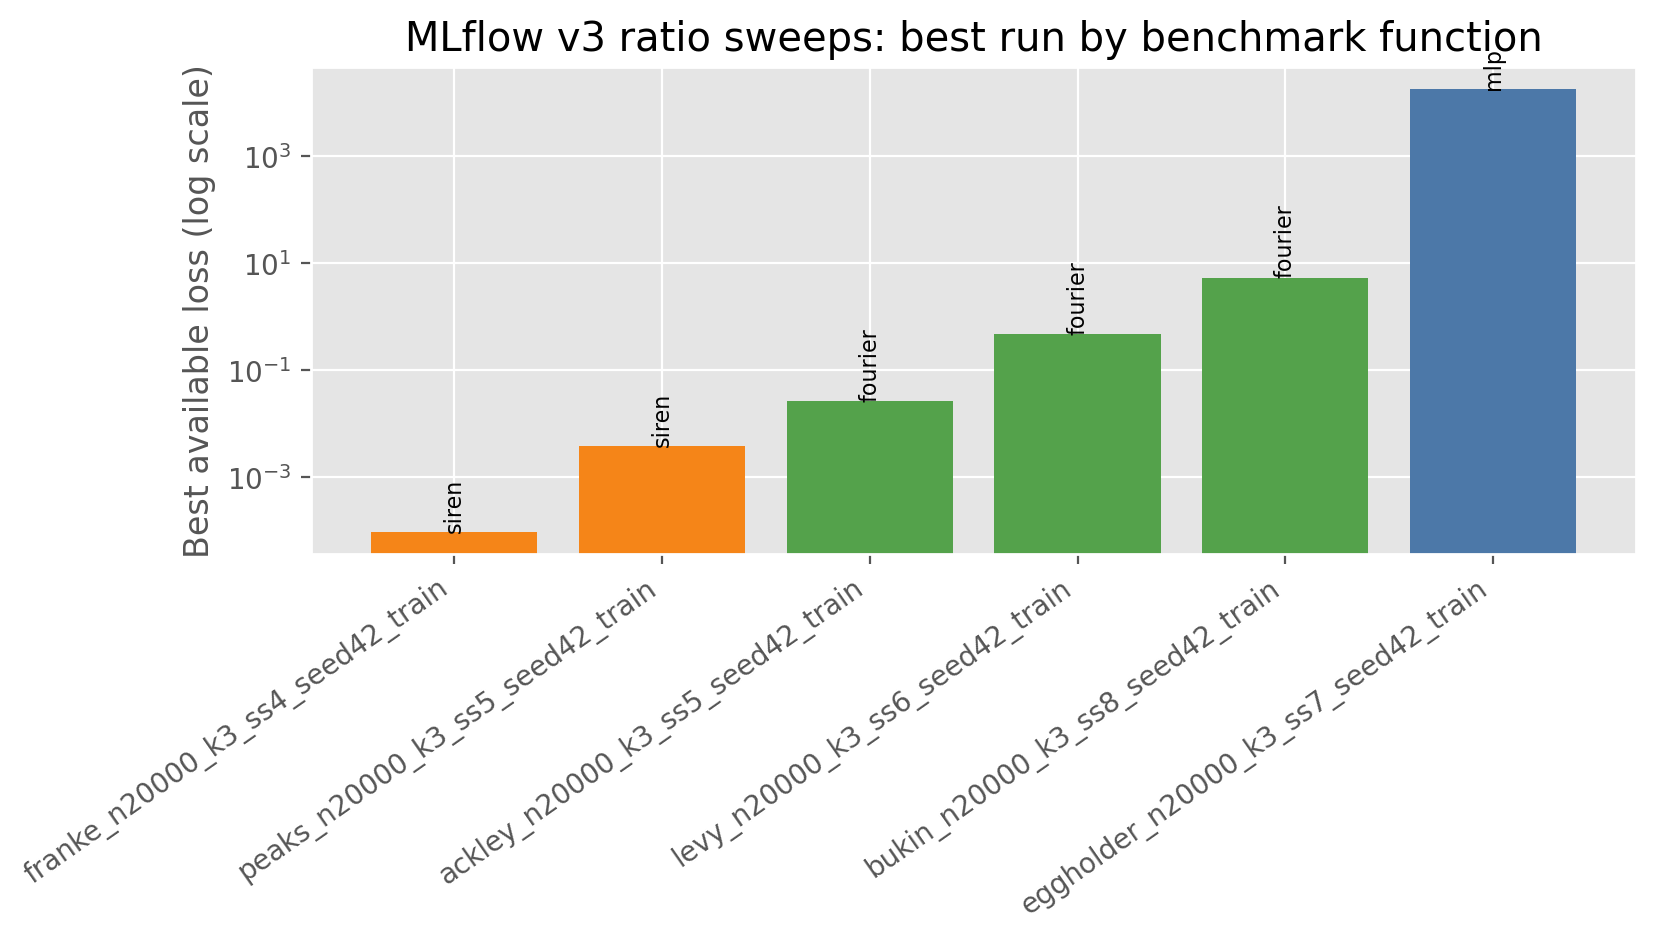
\includegraphics[width=0.86\textwidth]{figures/deep_mlflow_v3_best_losses.png}
    \caption{Best available loss from the v3 ratio-constrained MLflow sweeps.
    Bar labels show the architecture of the best trial.}
    \label{fig:deep-v3-best-losses}
\end{figure}

\begin{figure}[h]
    \centering
    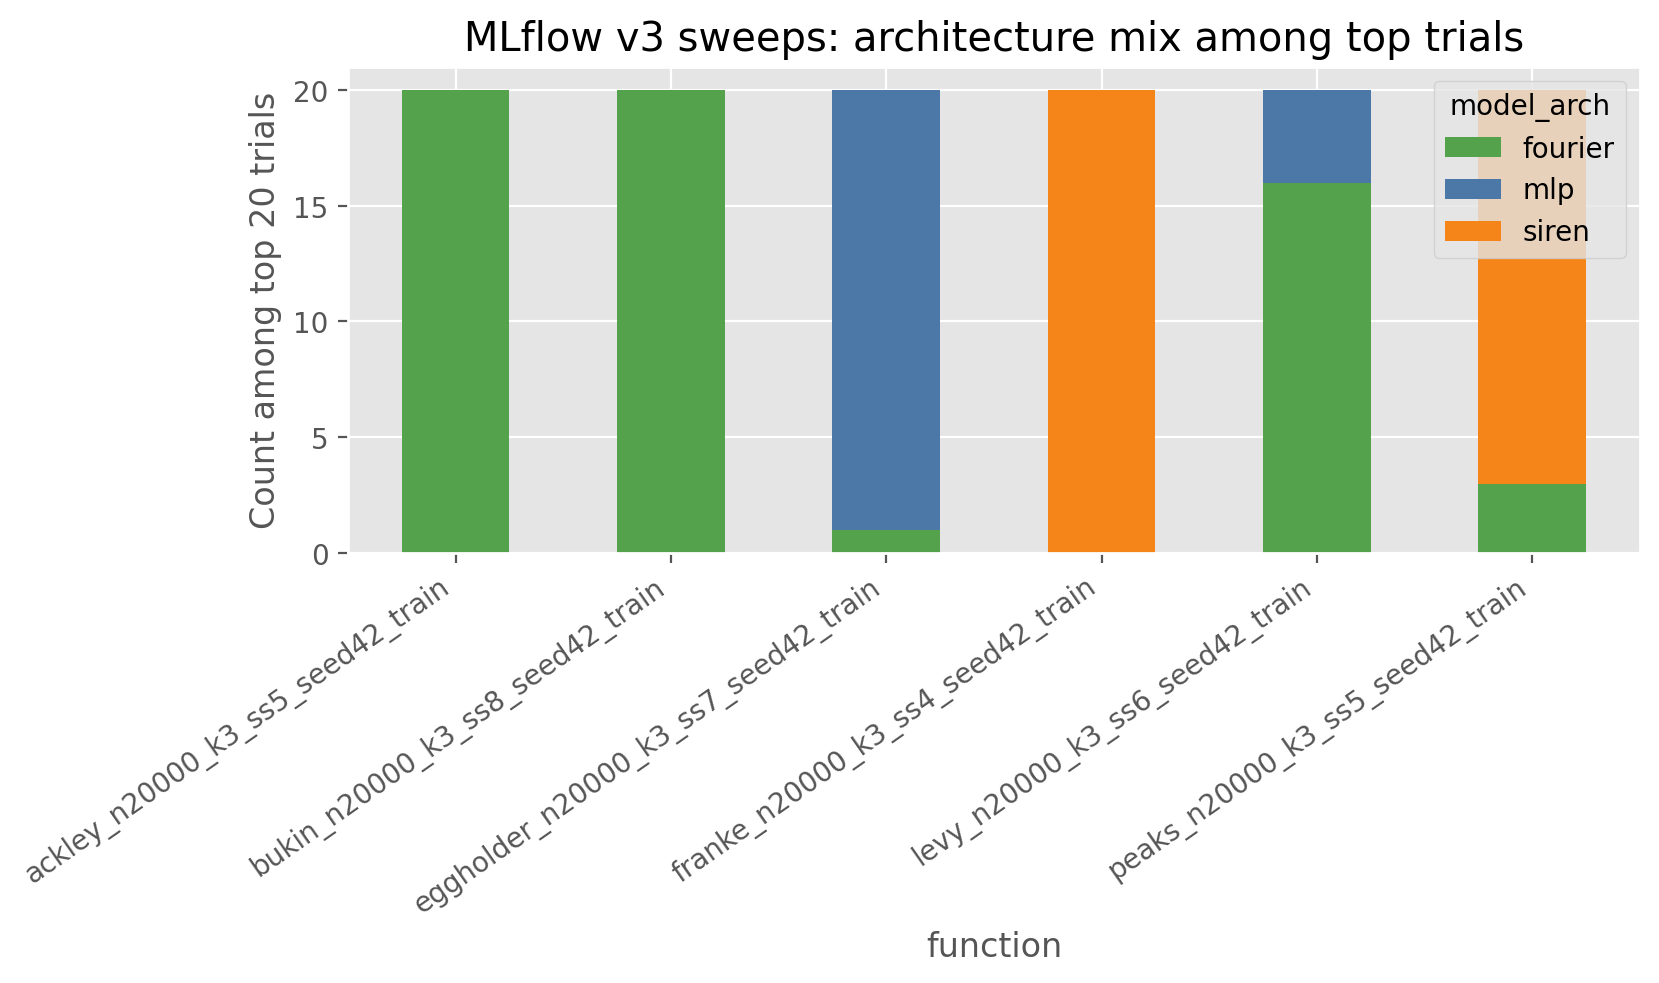
\includegraphics[width=0.86\textwidth]{figures/deep_mlflow_v3_top20_arch_distribution.png}
    \caption{Architecture composition among the top 20 v3 sweep trials per
    function. This is more informative than only reporting the single best trial,
    because it shows whether an architecture family is consistently competitive.}
    \label{fig:deep-v3-arch-distribution}
\end{figure}

\section{Exploratory schedule-policy search}

The repository also contains exploratory policy-schedule benchmarks for
\texttt{eggholder}. These are not as central as the controlled curriculum and
vision studies, but they are useful because they show that automatic schedule
search can find competitive regions while remaining noisy across seeds. Lower
loss is better.

\begin{table}[h]
\centering
\small
\begin{tabular}{lrrr}
\toprule
Schedule & Mean best hard-val loss & Std. & Mean epochs \\
\midrule
0003 & 0.5 & 0.3 & 100.0 \\
0004 & 1.6 & 1.2 & 100.0 \\
0005 & 2.1 & 1.9 & 95.7 \\
None & 2.1 & 1.9 & 95.7 \\
0002 & 2.3 & 1.5 & 94.7 \\
Optuna parametric schedule & 43670.0 & 11412.6 & 90.7 \\
\bottomrule
\end{tabular}
\caption{Top exploratory policy schedules and the best Optuna parametric
schedule when available. These runs are best read as schedule-search evidence,
not as final method comparisons.}
\label{tab:deep-policy-search}
\end{table}

\section{CIFAR-100 curriculum length and capacity}

Figure~\ref{fig:deep-cifar100-length} expands the model-size appendix by
showing every tested curriculum length as a gain over the matching baseline.
The within-family CNN pattern is especially clear: as width increases, the best
curriculum becomes shorter and eventually disappears.

\begin{figure}[h]
    \centering
    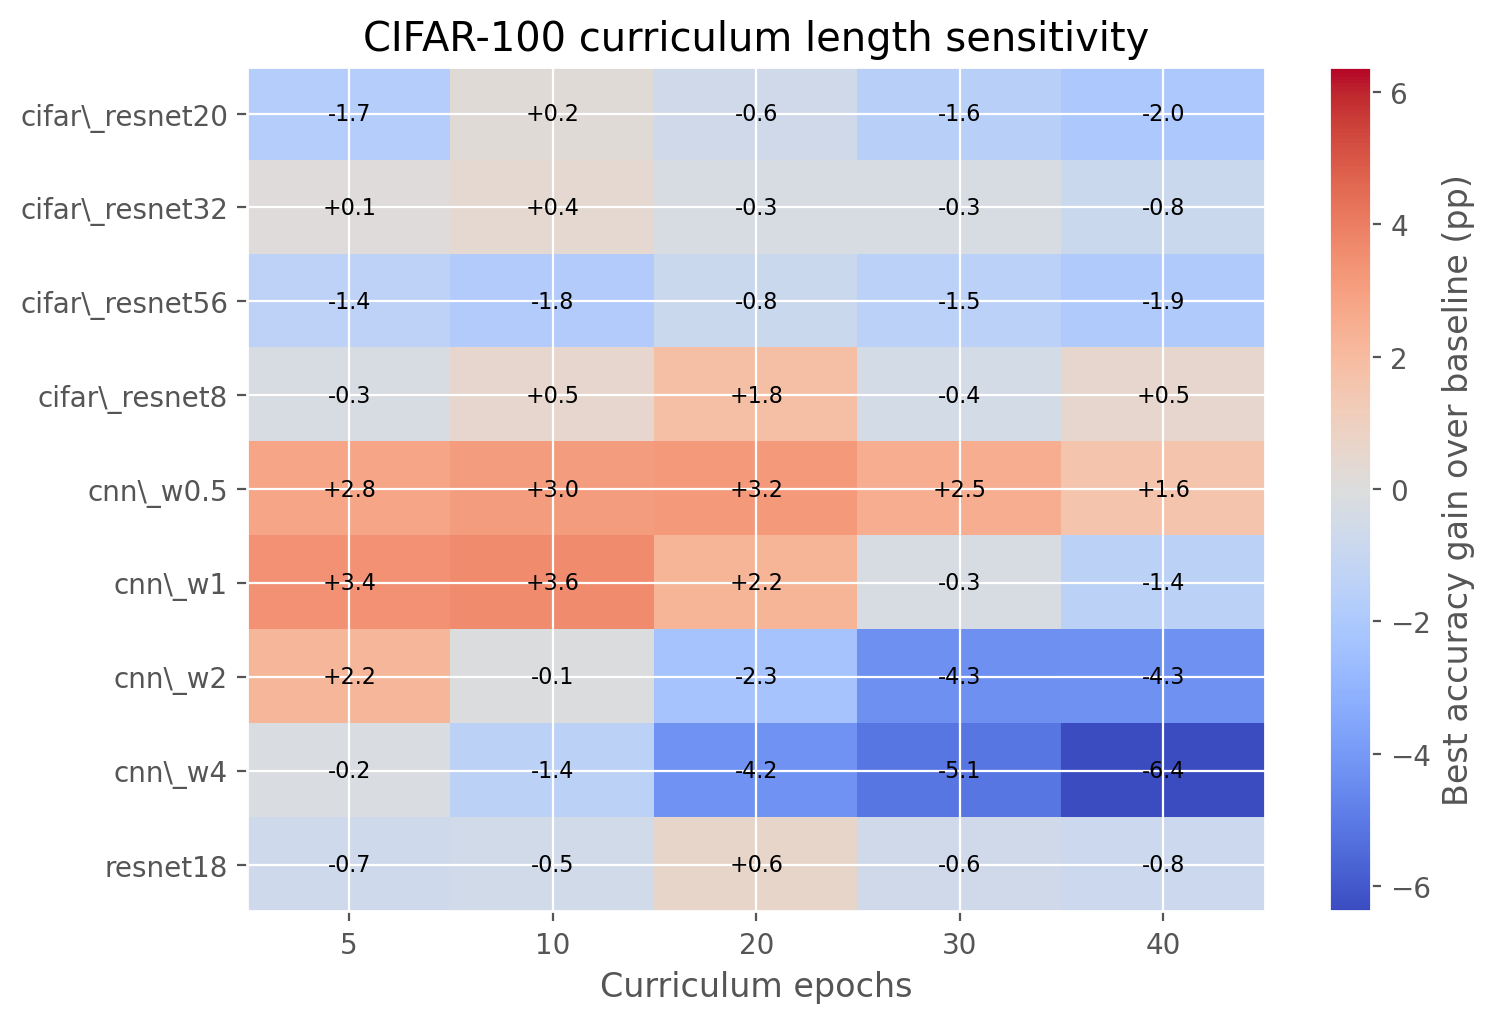
\includegraphics[width=0.86\textwidth]{figures/deep_cifar100_curriculum_length_heatmap.png}
    \caption{CIFAR-100 curriculum-length sensitivity. Values are best-test
    accuracy gains in percentage points relative to the matching baseline.}
    \label{fig:deep-cifar100-length}
\end{figure}

Figure~\ref{fig:deep-cifar100-milestones} asks when the best curriculum run is
above or below the baseline. Many curricula are below the baseline early and
recover later, which explains why peak accuracy and AUC tell different stories.

\begin{figure}[h]
    \centering
    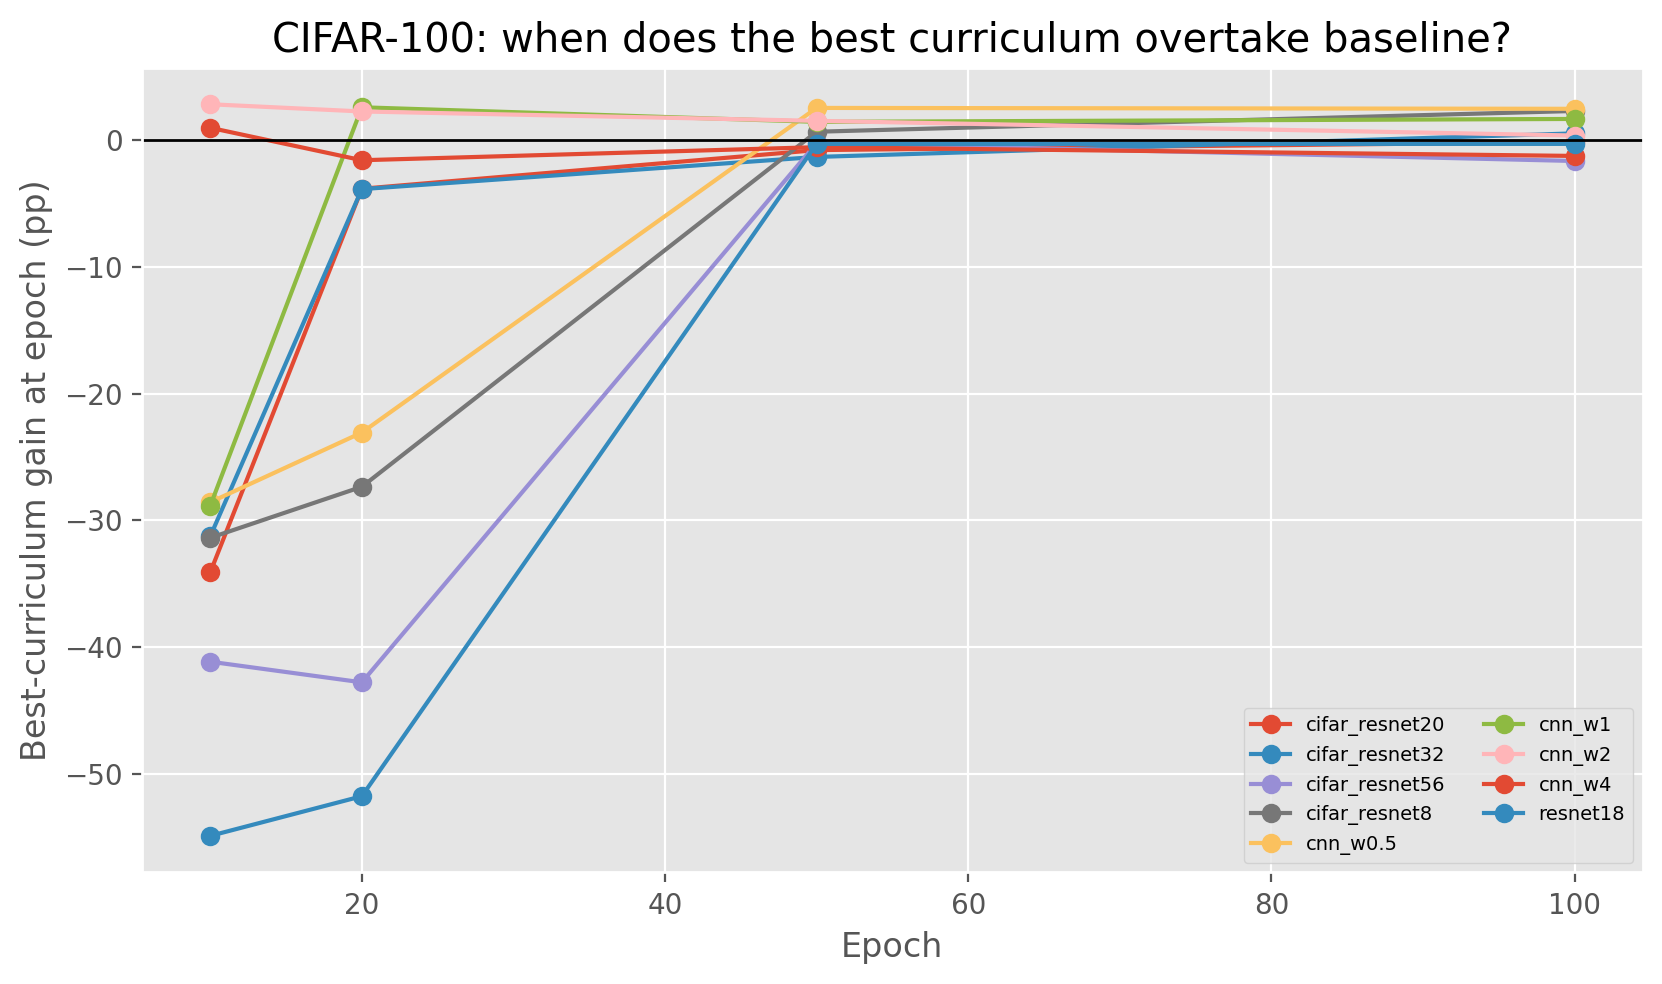
\includegraphics[width=0.86\textwidth]{figures/deep_cifar100_milestone_gains.png}
    \caption{Milestone test-accuracy gains of each model's best curriculum run
    relative to its baseline. Negative early values indicate the fine-label
    delay introduced by coarse training.}
    \label{fig:deep-cifar100-milestones}
\end{figure}

\begin{figure}[h]
    \centering
    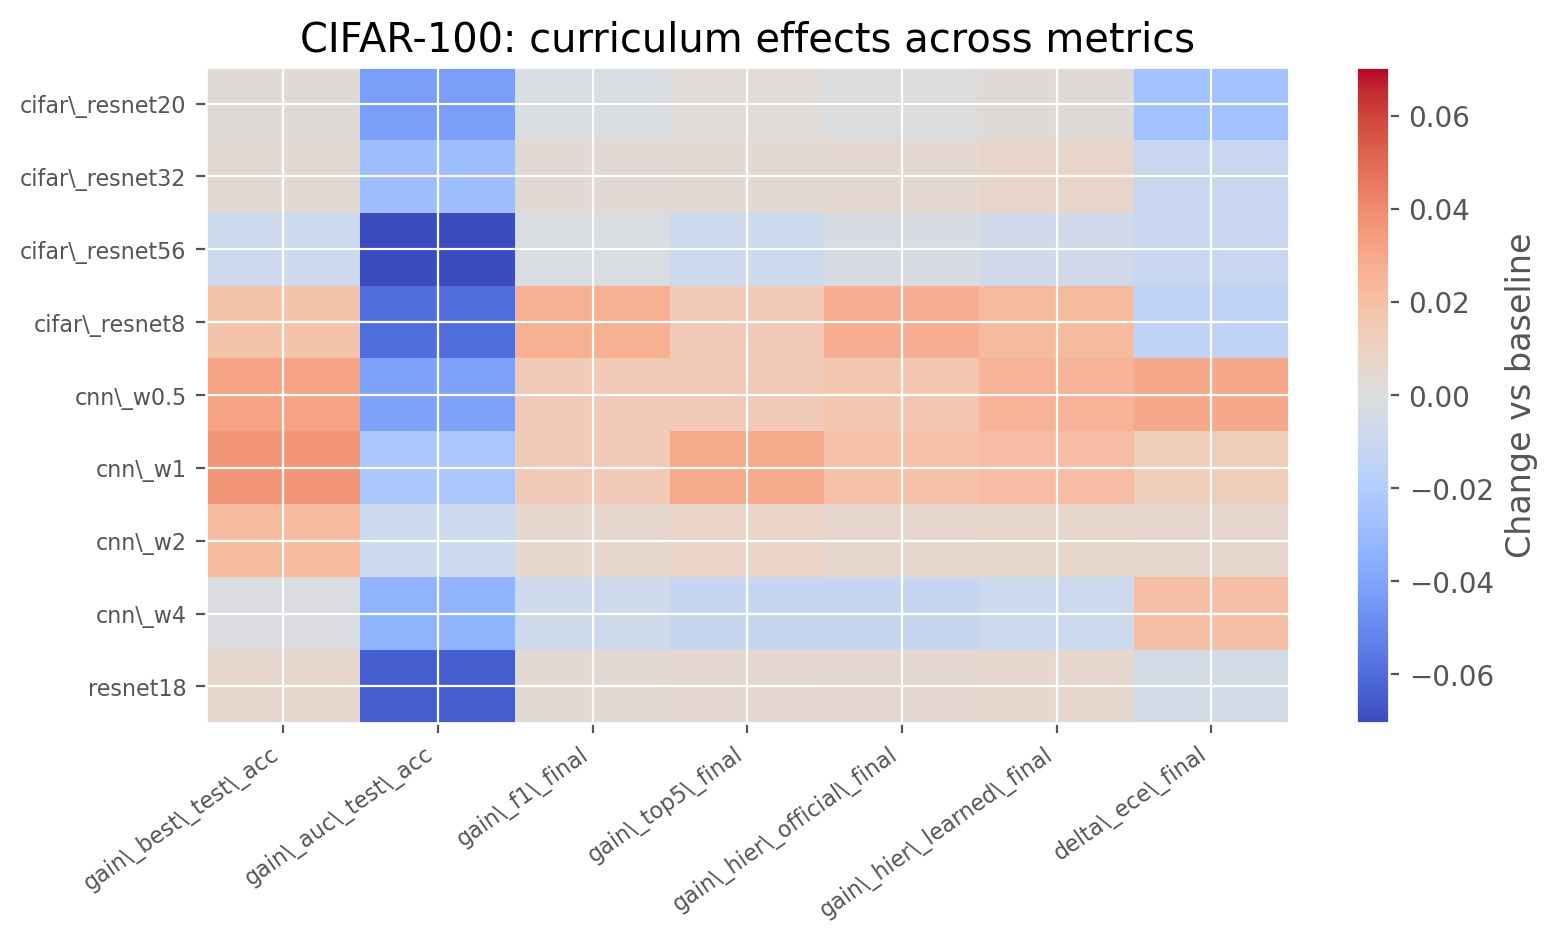
\includegraphics[width=0.86\textwidth]{figures/deep_cifar100_alt_metric_heatmap.png}
    \caption{CIFAR-100 metric heatmap for the best curriculum run of each
    model. Accuracy, macro-F1, top-5, hierarchy-aware scores, and calibration do
    not always move together.}
    \label{fig:deep-cifar100-alt-metrics}
\end{figure}

\section{Vision follow-up: gains, roughness, and schedule allocation}

Table~\ref{tab:deep-roughness-deltas} integrates the paired follow-up deltas
from the W\&B exports. The gain columns are reported in percentage points.
Negative AUC gains are common, reinforcing the interpretation that curricula can
improve the best solution reached while still delaying the fine-label trajectory.

\begin{table}[h]
\centering
\scriptsize
\begin{tabular}{lllrrrrr}
\toprule
Dataset & Model & Label & Best gain & AUC gain & ECE delta & Final sharp. & Final Hess. \\
\midrule
cifar10 & cifar\_resnet8 & curr10 & +0.09 & -3.61 & -0.48 & 0.56 & -0.04 \\
cifar10 & cnn\_w0.5 & curr10 & +0.24 & -2.80 & +0.98 & 0.23 & 0.16 \\
cifar10 & cnn\_w0.5 & curr20 & +0.78 & -6.75 & +0.34 & 0.12 & 0.19 \\
cifar100 & cifar\_resnet8 & curr20 & +1.33 & -1.96 & -1.44 & -0.16 & -0.30 \\
cifar100 & cnn\_w0.5 & curr20 & +2.54 & -1.72 & +4.73 & 0.03 & 0.03 \\
cifar100 & cnn\_w1 & curr10 & +1.98 & -0.23 & -0.01 & 0.35 & 0.04 \\
cifar100 & cnn\_w2 & curr5 & +1.72 & +0.15 & +0.14 & -0.08 & 0.06 \\
cifar100 & cnn\_w4 & curr5 & +0.34 & -1.03 & +0.42 & 0.15 & 0.23 \\
fashion-mnist & cifar\_resnet8 & curr10 & -0.42 & -7.43 & +0.61 & 0.05 & -0.38 \\
fashion-mnist & cnn\_w0.5 & curr10 & +0.11 & -5.91 & +0.63 & -0.14 & -0.62 \\
fashion-mnist & cnn\_w0.5 & curr20 & +0.12 & -12.01 & +0.40 & -0.10 & -0.41 \\
fashion-mnist & cnn\_w1 & curr10 & +0.12 & -6.45 & -0.12 & 0.20 & -0.01 \\
fashion-mnist & cnn\_w4 & curr5 & -0.16 & -3.25 & -0.10 & -0.16 & 0.32 \\
tiny-imagenet & cifar\_resnet8 & curr20 & -1.26 & -5.52 & +0.76 & -0.50 & 0.24 \\
tiny-imagenet & cnn\_w1 & curr20 & -7.23 & -5.71 & +2.79 & 0.08 & 0.20 \\
\bottomrule
\end{tabular}
\caption{Paired W\&B follow-up deltas by dataset, model, and curriculum label.
Sharpness and Hessian columns are log10 curriculum/baseline ratios; negative
values mean lower diagnostic value for curriculum.}
\label{tab:deep-roughness-deltas}
\end{table}

\begin{figure}[h]
    \centering
    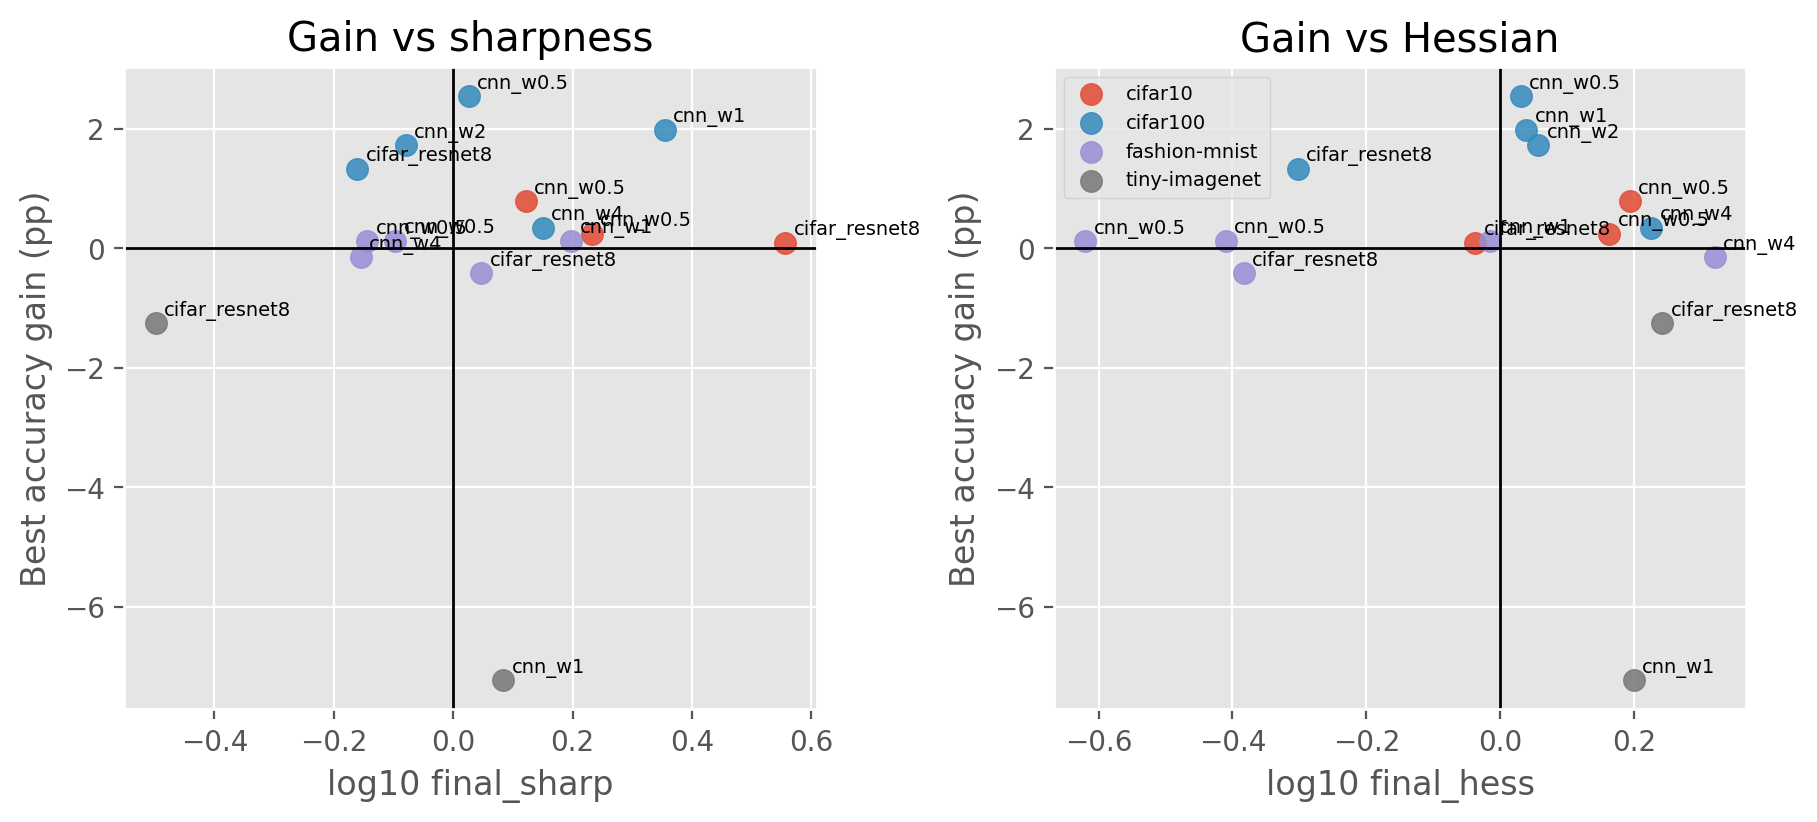
\includegraphics[width=0.92\textwidth]{figures/deep_roughness_gain_scatter.png}
    \caption{Relationship between best-accuracy gain and roughness diagnostics.
    The mixed pattern supports using roughness as a diagnostic, not as proof of a
    universal mechanism.}
    \label{fig:deep-roughness-scatter}
\end{figure}

\begin{figure}[h]
    \centering
    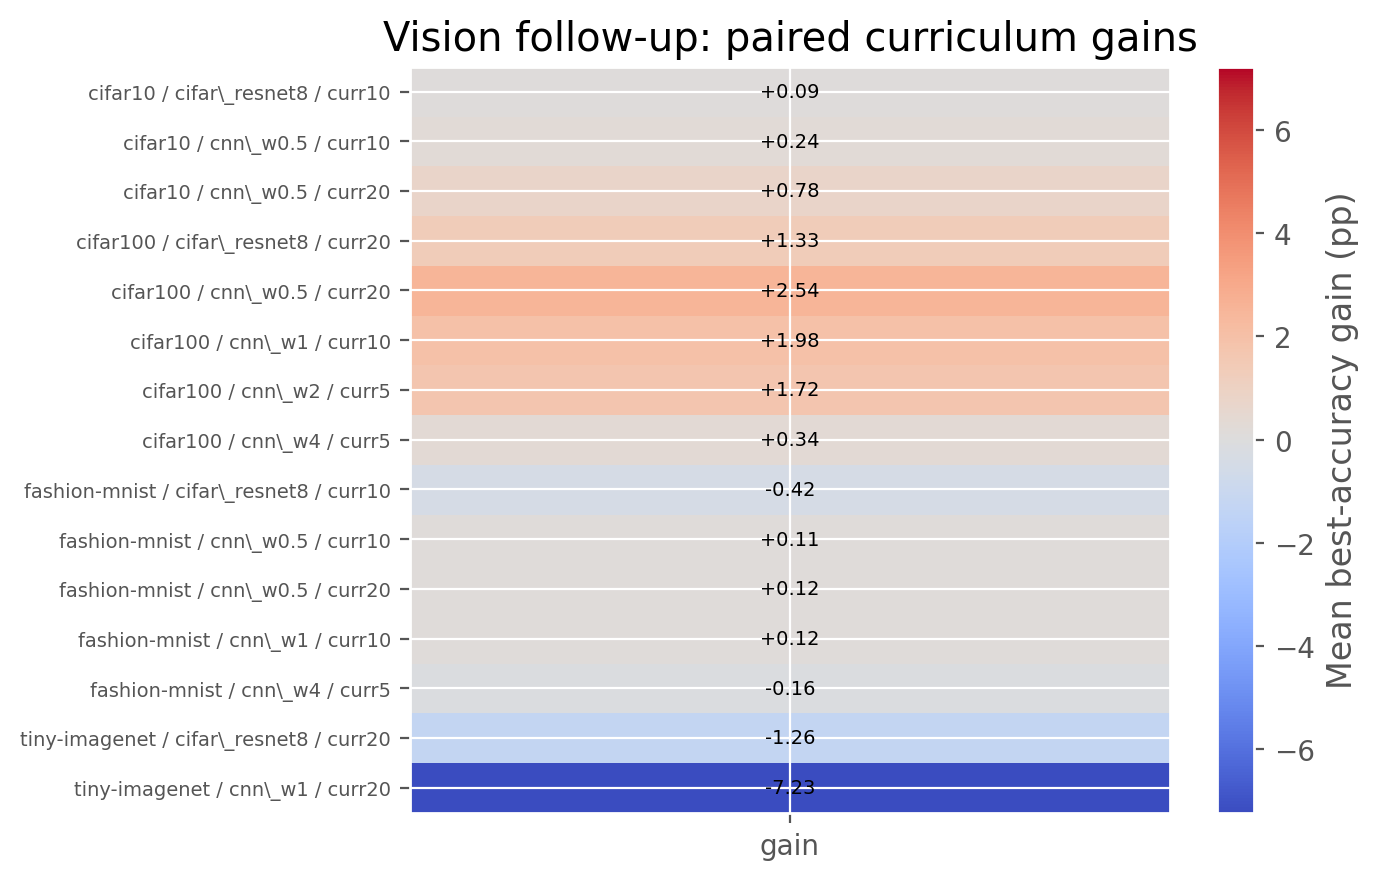
\includegraphics[width=0.74\textwidth]{figures/deep_vision_followup_gain_heatmap.png}
    \caption{Paired best-accuracy gains across all vision follow-up settings.}
    \label{fig:deep-vision-gain-heatmap}
\end{figure}

\begin{figure}[h]
    \centering
    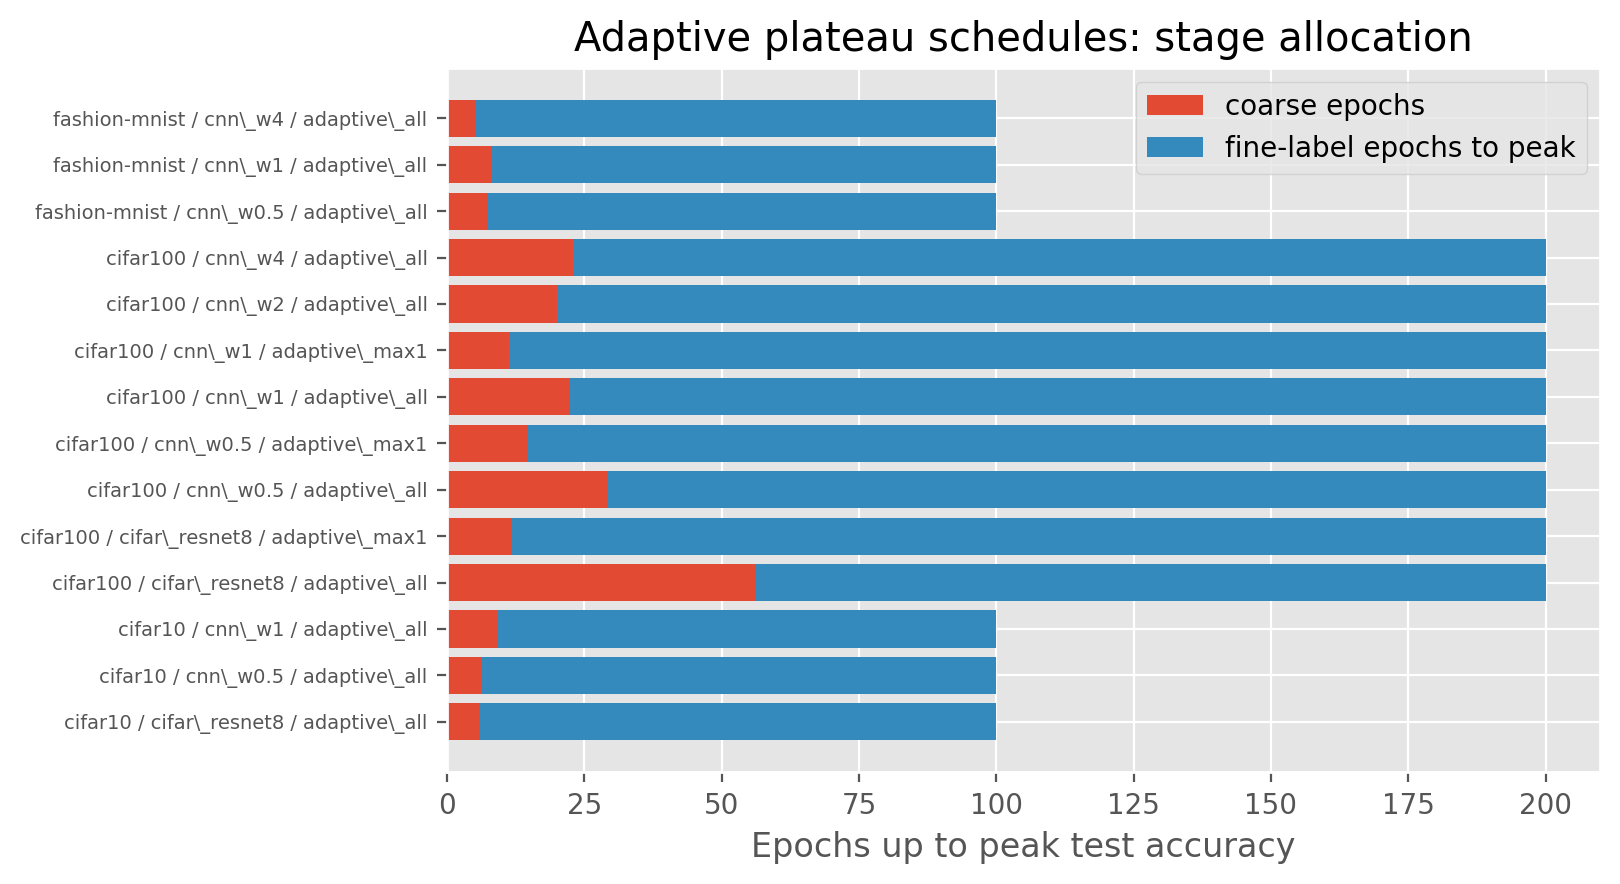
\includegraphics[width=0.86\textwidth]{figures/deep_adaptive_stage_allocation.png}
    \caption{Adaptive plateau stage allocation. Larger CIFAR-100 CNNs often
    spend too long in coarse stages relative to the short fixed curricula that
    worked best in the screening study.}
    \label{fig:deep-adaptive-stage-allocation}
\end{figure}

\section{Hierarchy ablation details}

Figure~\ref{fig:deep-hierarchy-seed-gains} shows the seed-level random-hierarchy
control. The learned hierarchy beats the random mean for every seed and also
beats the best random hierarchy tried for each seed. This is stronger than a
single aggregate number because it rules out the explanation that one lucky seed
created the learned-hierarchy advantage.

\begin{figure}[h]
    \centering
    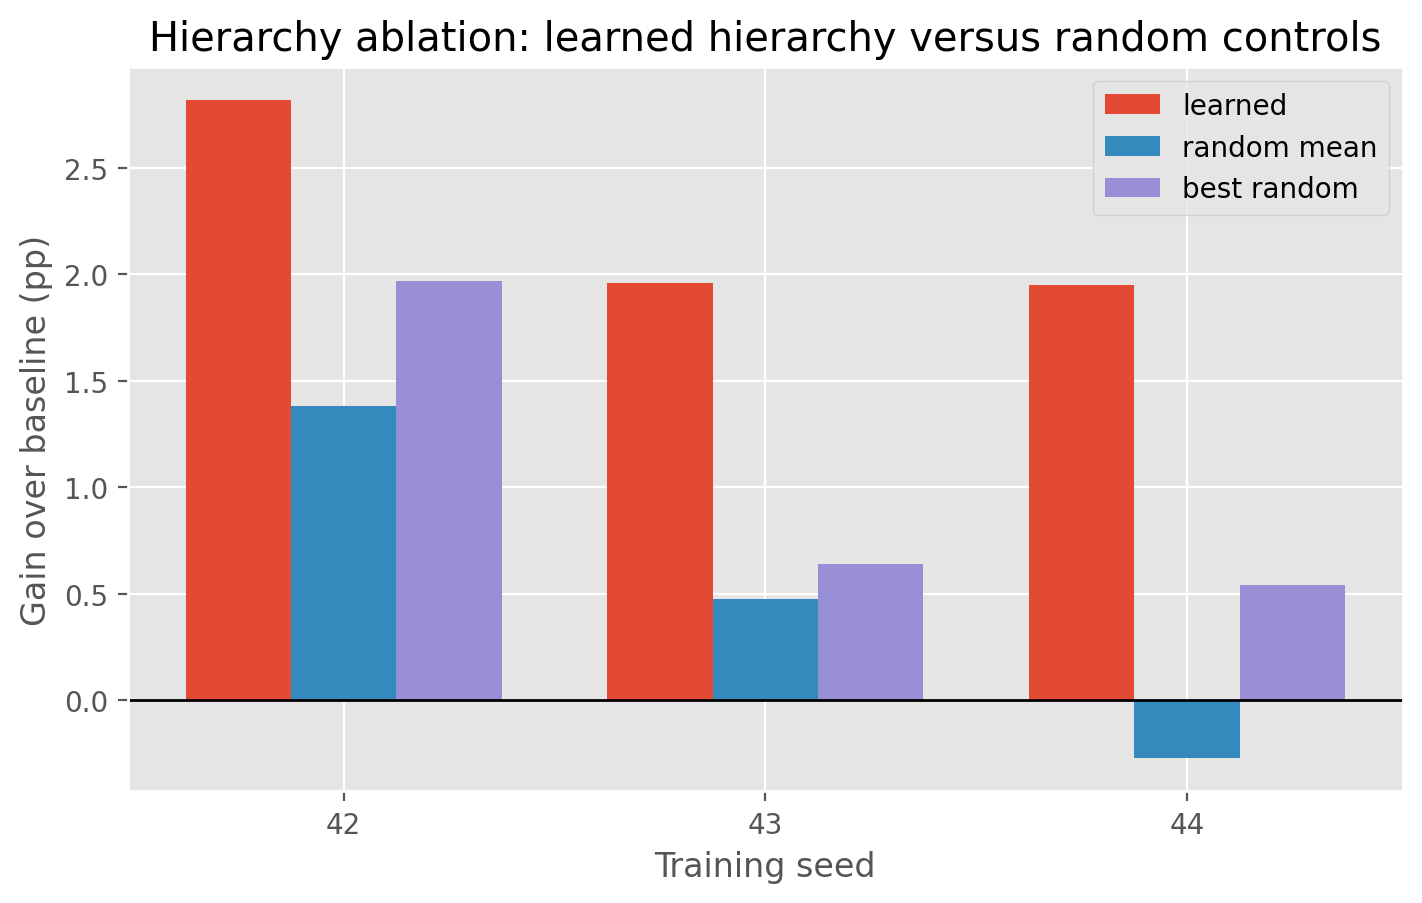
\includegraphics[width=0.78\textwidth]{figures/deep_hierarchy_seed_gains.png}
    \caption{Seed-level hierarchy ablation gains for CIFAR-100
    \texttt{cnn\_w0.5}.}
    \label{fig:deep-hierarchy-seed-gains}
\end{figure}

\section{What these additional plots suggest}

The deeper analysis strengthens four thesis-level points. First, the regression
track is genuinely mixed: continuation sometimes improves quality, but the
runtime cost is systematic. Second, the vision track has a clearer positive
region, but that region is bounded by capacity, schedule length, and dataset
structure. Third, adaptive schedules fail in an interpretable way: they often
allocate too many epochs to coarse objectives. Fourth, roughness diagnostics are
interesting but not decisive; they help characterize runs, but they do not yet
explain all positive curriculum effects.
